\documentclass[float=false, crop=false]{standalone}
\usepackage[subpreambles=true]{standalone}
\usepackage{import}

\usepackage{subfiles}
\usepackage[backend=biber,style=numeric,sorting=none]{biblatex}
\usepackage{import}

\renewcommand{\rmdefault}{bch} % change default font

\usepackage[english]{babel}
\usepackage[utf8]{inputenc}
\usepackage{tikz} 
\usetikzlibrary{arrows,decorations.pathmorphing,backgrounds,fit,positioning,shapes.symbols,chains}

\usepackage{amsmath}

\usepackage{csquotes}

\begin{document}
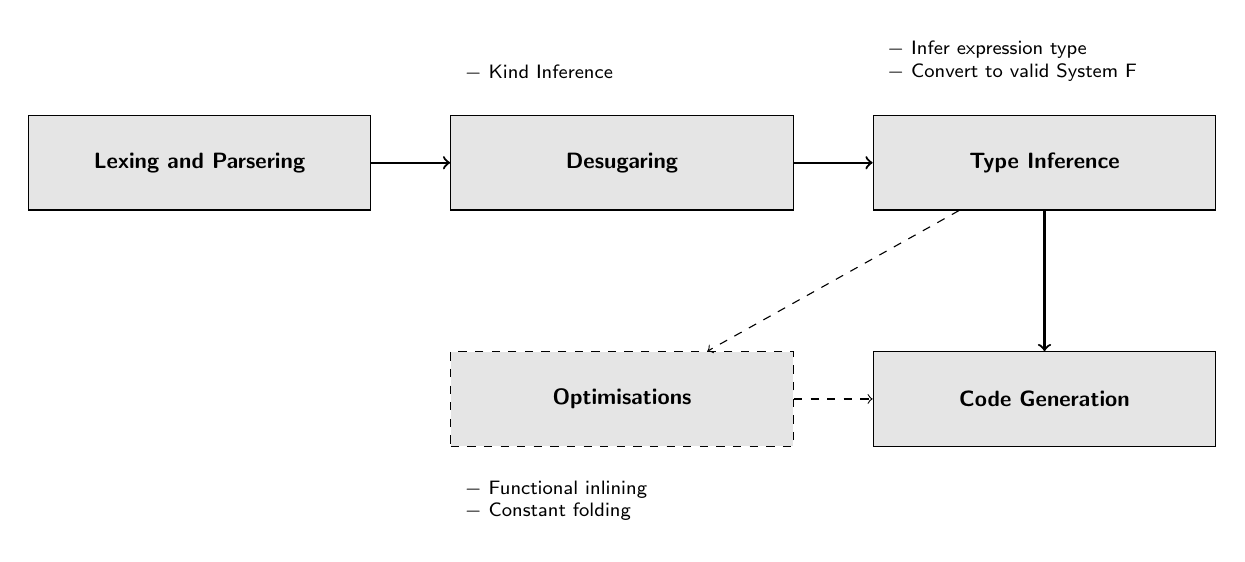
\begin{tikzpicture}
[node distance = 1cm, auto,font=\footnotesize,
% STYLES
every node/.style={node distance=3cm},
% The comment style is used to describe the characteristics of each force
comment/.style={rectangle, inner sep= 5pt, text width=4cm, node distance=0.25cm, font=\scriptsize\sffamily},
% The force style is used to draw the forces' name
force/.style={rectangle, draw, fill=black!10, inner sep=5pt, text width=4cm, text badly centered, minimum height=1.2cm, font=\bfseries\footnotesize\sffamily}] 

% Draw forces
\node [force] (lexparse) {Lexing and Parsering};
\node [force, right=1cm of lexparse] (desugar) {Desugaring};
\node [force, right=1cm of desugar] (ti) {Type Inference};
\node [force, below of=desugar, dashed] (opt) {Optimisations};
\node [force, right=1cm of opt] (codegen) {Code Generation};


%%%%%%%%%%%%%%%
% Change data from here

% Lex Parse
% \node [comment, above=0.25 of lexparse] (comment-lexparse) 
%   {Library -- Alex, Happy};

% Desguar
\node [comment, above=0.25cm of desugar] 
{ $-$ Kind Inference };

% % ti
\node [comment, above=0.25 of ti] {
  $-$ Infer expression type\\
  $-$ Convert to valid System F};

% % Optimization
\node [comment, below=0.25 of opt] 
{ $-$ Functional inlining\\
 $-$ Constant folding};

% % Code Generation
% \node [comment, below=0.25 of codegen] 
%   {$-$ Codec-JVM};


% %%%%%%%%%%%%%%%%

% % Draw the links between forces
\path[->,thick] 
(lexparse) edge (desugar)
(desugar) edge (ti)
(ti) edge (codegen);

\path[->,dashed]
(ti) edge (opt)
(opt) edge (codegen);

\end{tikzpicture} 
\end{document}
